\documentclass[a4paper,10pt]{article}
\usepackage[utf8]{inputenc}
\usepackage{fullpage}
\usepackage{cite}
\usepackage{graphicx}
\usepackage{wrapfig}
\usepackage{url}
\DeclareGraphicsExtensions{.pdf,.eps,.svg,.pgm}
    % EXTREMELY COMMON LaTeX PACKAGES TO INCLUDE:
    \usepackage{amsmath,amsthm, amsfonts,amssymb} % For AMS Beautification
    \usepackage{setspace} % For Single & Double Spacing Commands
    \usepackage[linktocpage,bookmarksopen,bookmarksnumbered,% For PDF navigation
		pdftitle={Group 2: Sotiriou et. al.},%   and URL hyperlinks
		pdfauthor={Department of Electronic and Computing Systems},%
		pdfsubject={UC },%
		pdfkeywords={UC}]{hyperref}
           \usepackage{caption3} % load caption package kernel first
    \DeclareCaptionOption{parskip}[]{} % disable "parskip" caption option
    \usepackage[small]{caption}
\usepackage{amsmath}
\usepackage{amsfonts}
\usepackage{amsthm}
%opening
\title{Assessing Histological Grades of Primary Breast Cancer Using Gene Signatures}
\author{Priyanka Arora, Lee Carraher,Ben Landis, Li Jing, Samuel Schmidt}
\begin{document}

\maketitle

\begin{abstract}
This paper is a re-Analysis of the Sotiriou et. al. paper on using tumor 
histological grade expressed gene signatures for breast cancer 
prognosis\cite{Sotiriou}. The principle assumptions of this process are that
the classification of histological grade and tumor progression has a strong 
correlation with the length of survival time. Furthermore, we suggest grade 2
tumors are misclassified grade 1 or grade 3 tumors. The result of developing 
better gene signatures for classifying tumor grades can further
assist in diagnosis and treatment options for breast cancer patients.


\end{abstract}

\section{Background}
\section{Purpose and Hypothesis}
\section{Methods and Materials}
\subsection{Data Acquisition and Sampling}
number of patients\\
datasets\\
tools and reagents\\
ER stuff\\
\subsection{Differential Expression Modeling Methods}
Our method of assessing histological grade of primary breast cancer consists of three phases. The first phase is
a semi-supervised ranking of genes and grade 1 and grade 3 tumors based on maximum differential
expression. The second phase consists of selecting a set of genes that are up-regulated with 
grade 3 tumors and down regulated in grade 3. In the third phase, we generated two groups of tumor samples.
Classification of the grade 2 tumors is then performed using these groups as models. Below we expand upon
our process in detail.\\
The gene signature identification process consisted of assessing the Sotiriou breast cancer data set with Genomics Portals (genomicsportals.org).
Genomics portals performs differential analysis on genes and samples using the CLEAN algorithm\cite{CLEAN}. CLEAN co-clusters
the genes and sample grades hierarchically, using data from the dataset and a database of known gene functional groups. Highly differentially
expressed genes were identified with a p-value of .001, and fold change over expression level of 2. The results of this analysis
were inspected in genomics portal's Treeview navigator\cite{Treeview}, and the visually most cohesive up-regulated set of genes
corresponding to grade 3 tumors was selected as our gene signature\ref{grade13diff}. Inspection with Treeview failed to suggested a 
visually significant cluster of down-regulated genes for grade 3 tumors, therefore only up-regulated ones were included in our model. 
We acquired a set of 49 differentially expressed up-regulated grade 3 tumor genes from this analysis.\\
\begin{figure}
\centering
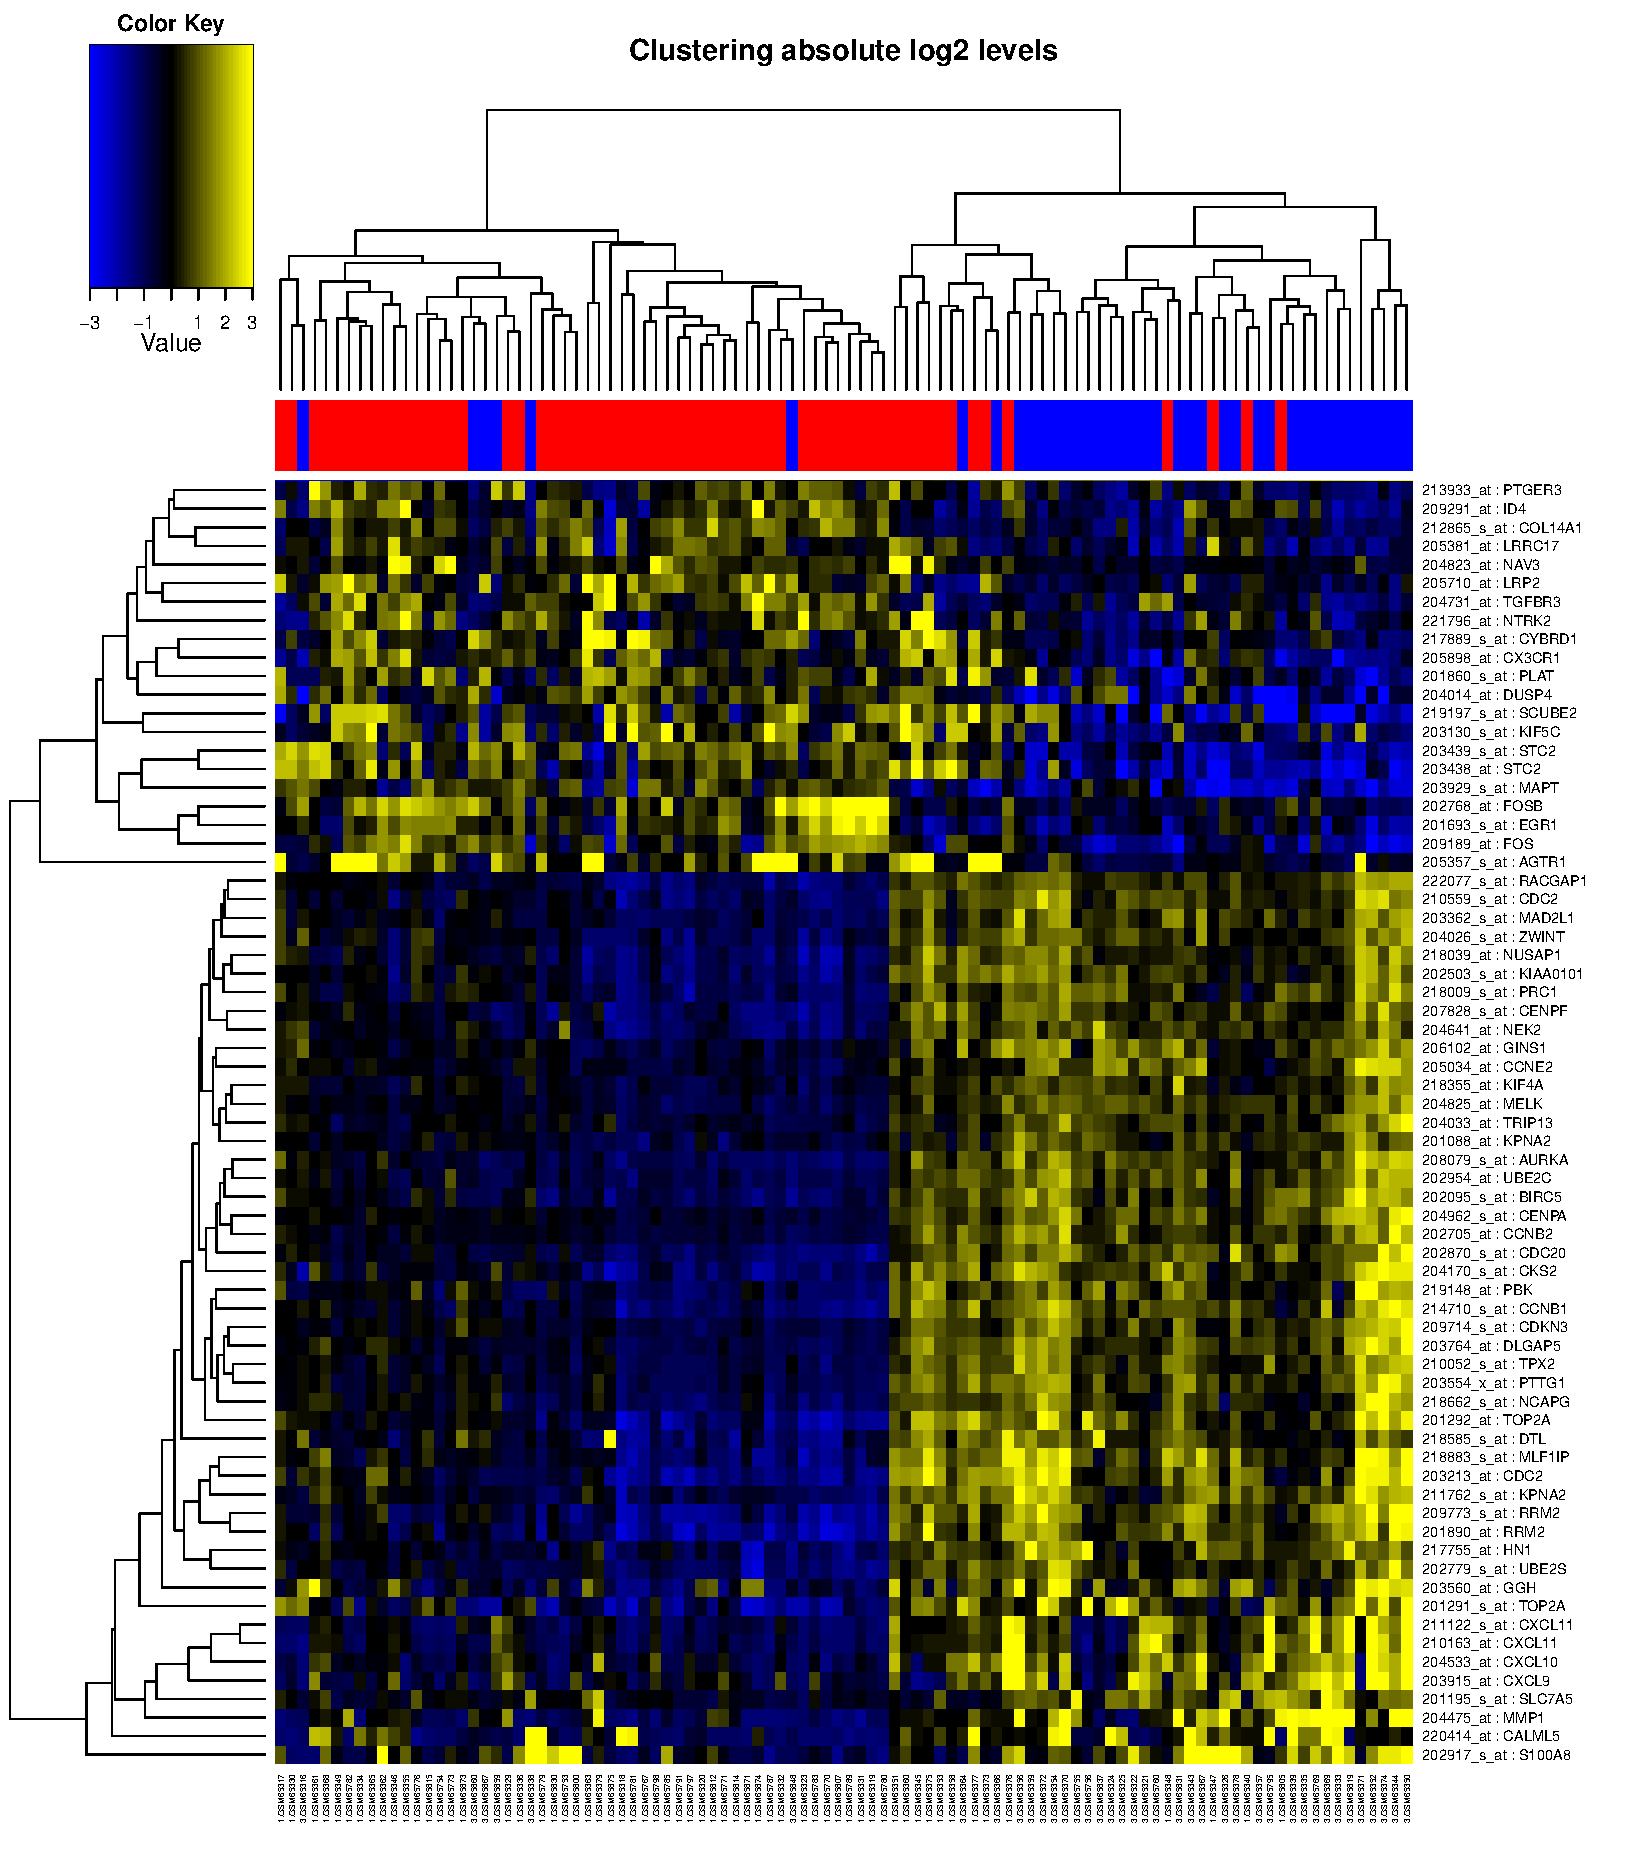
\includegraphics[scale=0.50]{docs/grade1and3differentiallyexpressed}
\caption{Grade 1 and Grade 3 Differentially Expressed}\label{grade13diff}
\end{figure}
Using the selected set of 49 genes as a signature we supposed a |gene signature|-dimensional subspace to build our model.
Withing the subspace, we used the clinically provided grade labels to generate centroids for the two , 1 and 3 - grade, groups following
the expression (Figure \ref{centroid}) . Noise suppression refinement was performed by removing samples that deviated from the group cluster
centers by more than 2 standard deviations of the cluster's mean variance.\\
\begin{figure}
$$
Centroid(Grade_X)= \left[              \underset{x\in X}     \sum{  { {x_1}    \over {| X |} } }   ,   
 \underset{x\in X}     \sum{  { {x_2}    \over {| X |} } },
\ldots ,
 \underset{x\in X}     \sum{  { {x_{| gene signature |}}    \over {| X |} } }                 \right] 
$$
\caption{Grade Gene Expression Centroid Generation}\label{centroid}
\end{figure}
For visual assessment of our analysis, we queried the grade 2 tumors against the grade 1 and 3 differentially expressed genes. The resulting chart
shows a distinct clustering between the grade 1-like and grade 3-like tumors that follow approximately 
the grade 3 and grade 1 distributions. Assuming the dataset comprises the actual distribution 
of grade 1 to grade 3 tumors, approximately 55:64 for grade 1 and grade 3 respectively (figure \ref{grade2up}) we reassert our hypothesis
of the lack of a grade 2 class distinction.
\begin{figure}
\centering
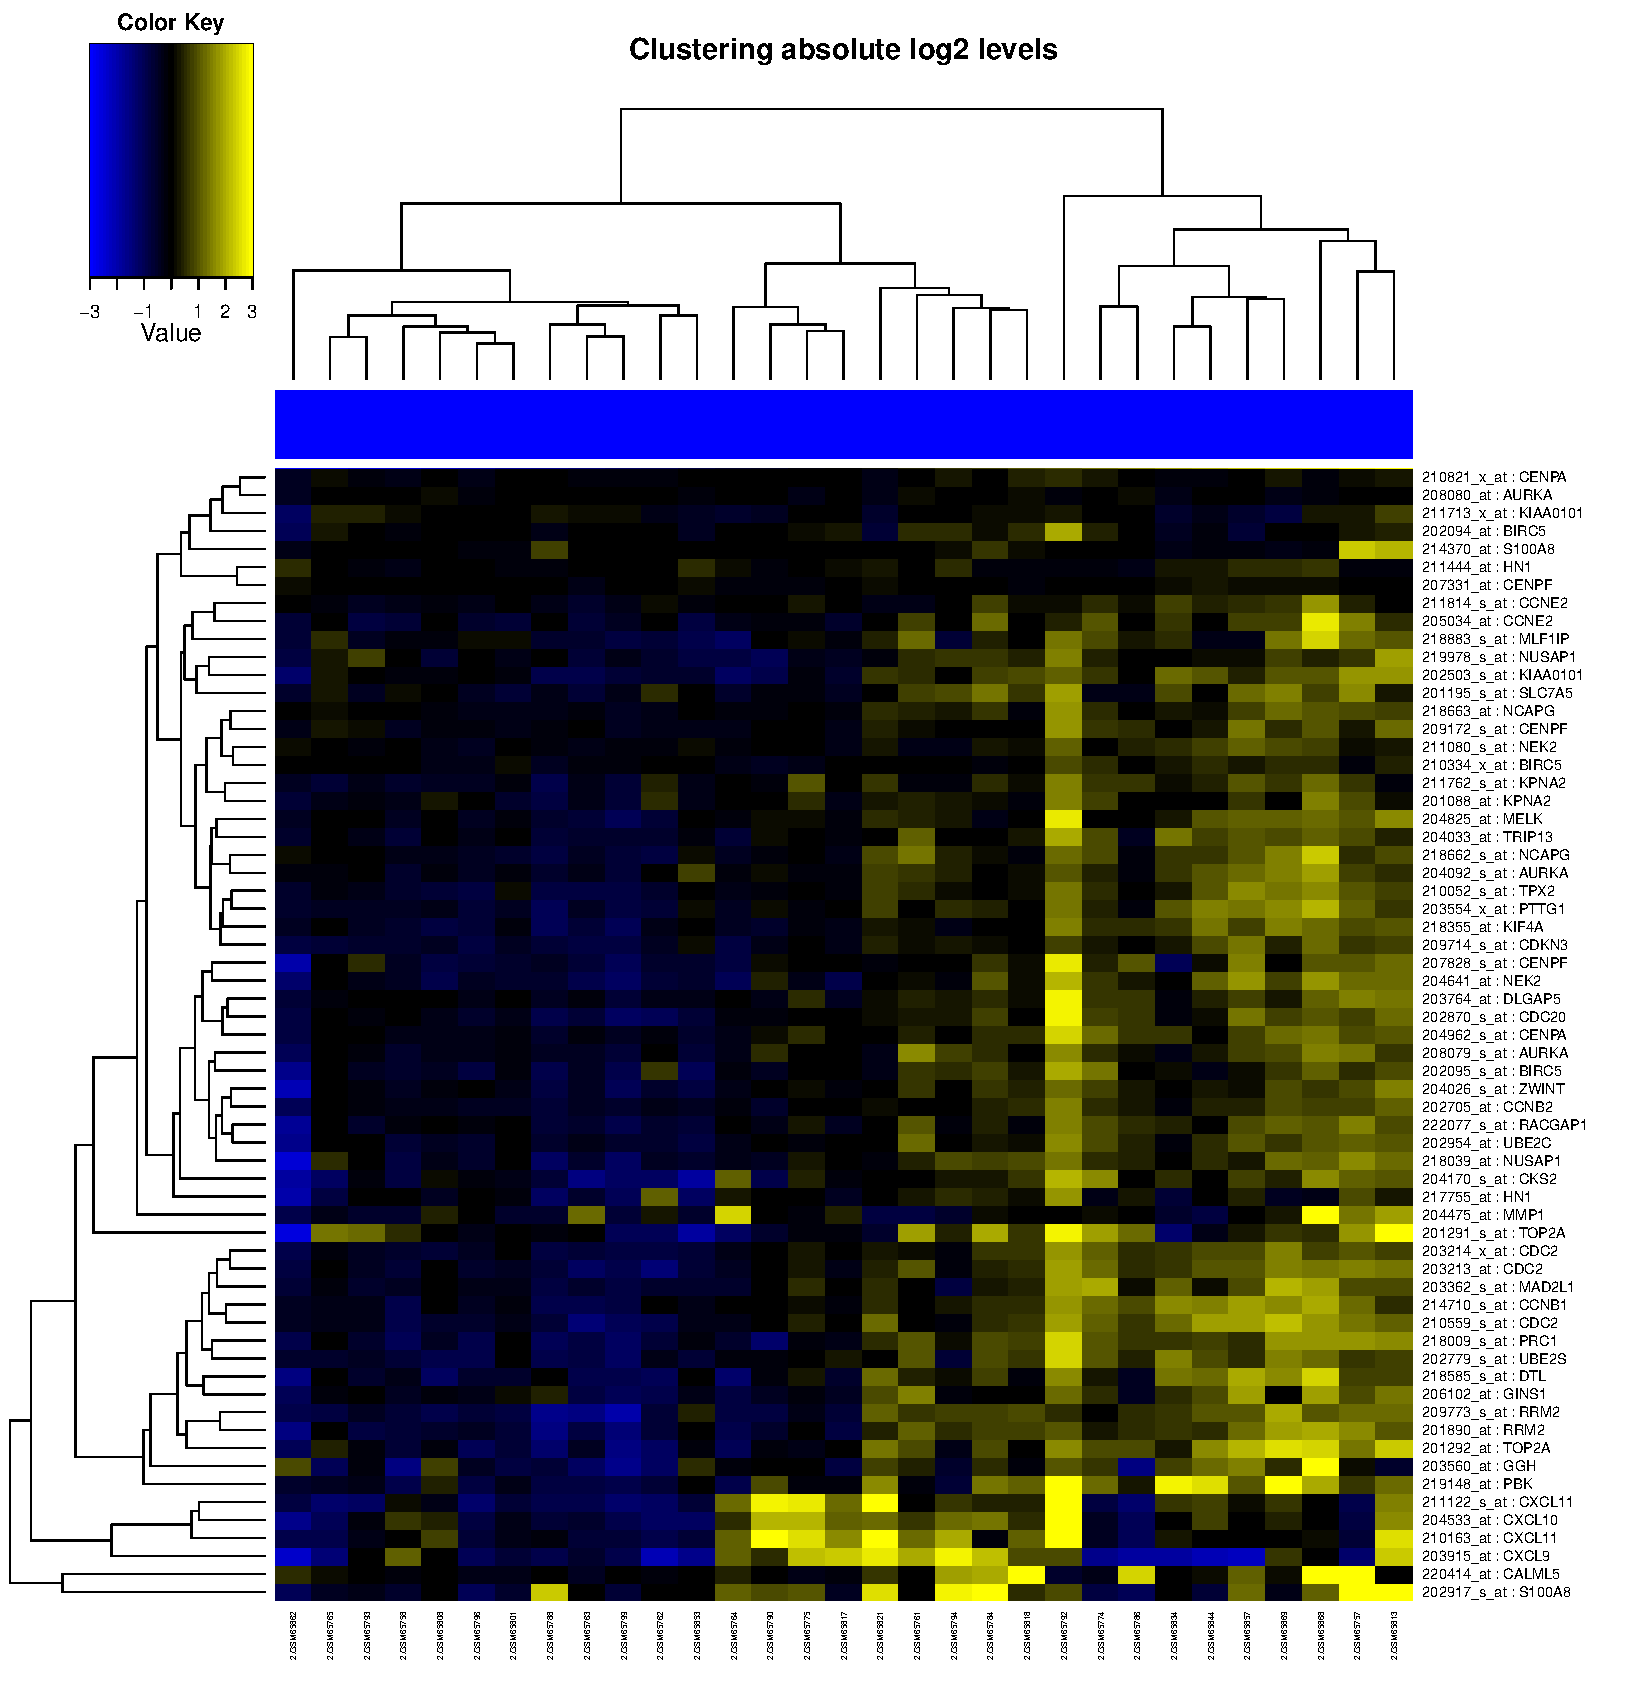
\includegraphics[scale=0.50]{docs/grade2onupregulated3}
\caption{Grade 2 Differentially Expressed Genes from Grade 1 and Grade 3}\label{grade2up}
\end{figure}

Classification of grade 2 tumors was then computed by nearest centroid under the euclidean norm following the method in figure \ref{classify}.
The new classifications were then used to recompute the KM-Survival analysis on tumor grades 2A (or grade 1-like) and 2b (or grade 3-like).

\begin{figure}
 $$
Grade(X) = \underset{C \in Centroids} {\mathrm{argmin}} ~ \left( \sqrt{\sum_{g\in genelist}{ (X_{g} - C_{g})^2}}\right)
$$
\caption{Nearest Centroid Classification}\label{classify}
\end{figure}



Computed centroids for grades 1 and 3 based on the 49 up-regulated genes identified with genomic portals.\cite{Treeview},\cite{CLEAN}

Used those centroids to reclassify grade 2 tumors using Nearest Centroid based on Euclidean distance.

* Projection to Latent Space Regression (PLSR) on 49, 7231, and 11467 genes.
 on 50:50 train, test data. 
* Identifies 6 genes: 2 calcium related proteins and 4 chemokines
* Unsupervised k-means was
  applied, with similarly poor classification     performance.
* Performed similar analysis with PAM50 
* Qualitatively the heatmap results were worse, as PAM50 is for subtype classification.
* Interestingly, nearest centroid assignment was almost identical.
Up-regulated genes from grade 3 and 1 differential expression applied to grade 2 tumors (Figure \ref{grade2up})

\section{Results and Discussion}
\section{Conclusion}
90\% of the time it works all the time!
\bibliography{refs}
\bibliographystyle{ieeetr} \markright{ }


\end{document}
